% Tipo de documento
\documentclass[12pt,a4paper]{article}

% Pacotes
%\usepackage{showlabels}
\usepackage{latexsym}
\usepackage{amsfonts}
\usepackage{amsmath}
\usepackage{amscd}
\usepackage[brazil]{babel}
\usepackage[utf8]{inputenc}
\usepackage[pdftex]{graphicx} 

% Paginação
%\textwidth 15.0cm                    % Largura
%\textheight 22.0cm                   % Altura
%\addtolength{\oddsidemargin}{0.0cm}  % Margem esquerda (impar)
%\addtolength{\evensidemargin}{0.0cm} % Margem esquerda (par)
%\addtolength{\topmargin}{0.0cm}      % Margem superior

% Estilo dos parágrafos
\sloppy                              % Mais flexível
\setlength{\jot}{08pt}               % Distância entre linhas do eqnarray
\setlength{\parskip}{1ex}            % Distância entre parágrafos
\renewcommand{\baselinestretch}{1.0} % Distância entre linhas

% Contagem de equações por seção
\renewcommand{\theequation}{\thesection.\arabic{equation}}

% Contagem de figuras por seção
\renewcommand{\thefigure}{\thesection.\arabic{figure}}

% Contagem de tabelas por seção
\renewcommand{\thetable}{\thesection.\arabic{table}}

% Zerar as contagem em cada seção
\newcommand{\zerar}{\setcounter{equation}{0}\setcounter{figure}{0}\setcounter{table}{0}}

\DeclareMathOperator{\col}{col}
\DeclareMathOperator{\row}{row}

% Conjunto de números
\newcommand{\Z}{\mathbb{Z}}
\newcommand{\C}{\mathbb{C}}
\newcommand{\N}{\mathbb{N}}
\newcommand{\Q}{\mathbb{Q}}
\newcommand{\R}{\mathbb{R}}

%%%%%%%%%%%%%%%%%%%%%%%%%%%%%%%%%%%%%%%%%%%%%%%%%%%%%%%%%%%%%%%%%%%%%%%%%%%%%%%%%%%%%%%%%%%%%%%%%%%%

\begin{document}

\title{{\sc MAC0425 -- Inteligência Artificial} \\ \vspace{0.5cm} {\bf Mina de Ouro}}
\author{Daniel Augusto Cortez}
\date{\today}

\maketitle

\begin{abstract}
Relatório descrevendo implementação e resultados do EP1 de Inteligência Artificial, IME-USP 2013
(Mina de Ouro).
\end{abstract}

%%%%%%%%%%%%%%%%%%%%%%%%%%%%%%%%%%%%%%%%%%%%%%%%%%%%%%%%%%%%%%%%%%%%%%%%%%%%%%%%%%%%%%%%%%%%%%%%%%%%

\zerar
\section{Introdução}
\label{sec:intro}

Este relatório descreve a minha implementação do EP para resolver o problema da mina de ouro 
proposto no enunciado, bem como oferece informações sobre testes e análise de desempenho das 
diferentes buscas.

A implementação foi escrita em Java (1.6.29) no ambiente de desenvolvimento Eclipse (Kepler) 
utilizando o sistema operacional Mac OS (10.7.2).

O código fonte (classes Java) se encontra no diretório \verb|/src/dacortez/minaDeOuro|. Uma versão 
compilada do programa \verb|minaDeOuro.jar| está disponível no diretório raiz junto com alguns 
arquivos de entrada. A utilização do programa se faz através da linha de comando:
%
\begin{verbatim}
$ java -jar minaDeOuro.jar <arquivo_de_entrada> <tipo_de_busca>
\end{verbatim}
%
Os tipos de busca suportados são:
%
\begin{verbatim}
  P: busca em profundidade limitada
  L: busca em largura
  A: busca A*
  U: busca uniforme
\end{verbatim}

%%%%%%%%%%%%%%%%%%%%%%%%%%%%%%%%%%%%%%%%%%%%%%%%%%%%%%%%%%%%%%%%%%%%%%%%%%%%%%%%%%%%%%%%%%%%%%%%%%%%

\zerar
\section{Estrutura de Classes}
\label{sec:classes}

A implementação foi realizada modularizando o programa em 15 classes, conforme descrição abaixo
(com comentários sobre os principais métodos de cada classe). A documentação completa (Javadoc) está
disponível no diretório \verb|/doc|.

\begin{itemize}

  \item{\verb|Main.java|}: Ponto de entrada do programa. Cria o objeto \verb|Enviroment| apropriado 
  a partir do arquivo de entrada e instância o tipo de agente escolhido. O objeto \verb|Environment| 
  pode ser acessado estaticamente pois é único ao longo da vida do agente. Os tipos de agente que 
  podem ser instanciados efetuam busca em largura limitada, busca em profundidade, busca A* e busca 
  uniforme.

  \item{\verb|Environment.java|}: Representa o ambiente da mina, contendo um mapa com suas posições 
  livres, obstruídas e com pepitas de ouro. Possui métodos que permitem ao agente decidir como se 
  mover ou se é possível pegar ouro. O método \verb|performanceMeasurement()| avalia a performance 
  do agente ao tomar a ação passada. Caso a ação seja pegar ouro, retorna $4n$, onde $n$ é a 
  dimensão da mina. Caso contrário, retorna -1. 

  \item{\verb|Agent.java|}: O agente é responsável por efetuar o procedimento de busca adequado
  na mina. O método de busca da solução \verb|getSolution()| é abstrato e deve ser implementado pela 
  instância concreta do agente que deriva desta classe. A estrutura comum a todos esses agentes, 
  entretanto, estão presentes nesta classe base.

  O principal método do agente é \verb|search()| que, a partir da estratégia de busca do agente, 
  explora a mina tentando coletar $1, 2, \ldots,$ todas as pepitas da mina, retornando a melhor
  solução possível.

  \item{\verb|AStarAgent.java|}: Este agente implementa o método de busca A*. É uma classe abstrata
  dericada de \verb|Agent|. As classes concretas devem implementar a função heurística. A 
  implementação do método \verb|getSolution()| é baseada no código \verb|GRAPH-SEARCH| 
  de~\cite{aima} utilizando uma fila de prioridades para os nós baseada na alaviação da função 
  $f(n) = g(n) + h(n)$.

  \item{\verb|AStarAgentHNearst.java|}: Concretiza a classe \verb|AStarAgent| utilizando uma 
  heurística que encontra as pepitas mais próximas do agente, uma a uma, e depois retorna à posição 
  inicial. Falaremos mais sobre a heurística utilizada na Seção~\ref{sec:h}.

  \item{\verb|AStarAgentHZero.java|}: Concretiza a classe \verb|AStarAgent| utilizando uma 
  heurística nula, o que equivale fazer a busca uniforme. Ou seja, esse agente implementa a busca 
  uniforme. 

  \item{\verb|BreadthAgent.java|}: Concretiza a classe \verb|Agent| implementando o método de busca 
  em largura. A implementação do método \verb|getSolution()| é baseada no código \verb|GRAPH-SEARCH|
  de~\cite{aima} utilizando uma fila FIFO padrão.

  \item{\verb|LimitedDepthAgent.java|}: Este agente implementa o método de busca em profundidade 
  limitada. A implementação do método \verb|getSolution()| é baseada no código recursivo
  \verb|DEPTH-LIMITED-SEARCH| de~\cite{aima}.
  
  \item{\verb|Position.java|}: Representa uma posição na mina como o par ordenado (linha, coluna).
  A posição (0, 0) corresponde ao canto superior esquerdo. Os valores de linha crescem para baixo e 
  os valores de coluna crescem para direita. Sobrescreve o método \verb|equals()| para se poder
  comparar instâncias diferentes de posições pelos valores de linha e coluna.

  \item{\verb|Action.java|}: Enum que define as ações que o agente pode executar na mina:
  %
  \begin{verbatim}
    RIGHT: mover para direita.
     LEFT: mover para esquerda.
     DOWN: mover para baixo.
     PICK: pegar ouro.
  \end{verbatim}
  %
  O método \verb|toString()| retorna uma String descritiva da ação para ser utlizada na impressão da 
  solução.
  
  \item{\verb|State.java|}: Representa o estado onde se encontra o agente em sua busca. O estado é 
  representado pela posição do agente e uma lista das posições das pepitas de ouro recolhidas.
  O principal método da classe é \verb|getSuccessors()| que representa a função sucessora para o 
  estado atual. O método \verb|equals()| foi sobrescrito para permitir comparação entre instâncias
  diferentes de estado baseada na posição do agente e na lista de pepitas coletadas.
  
  \item{\verb|ActionState.java|}: Representa um par (action, state), onde o estado state é atingido 
  após a execução da ação action.

  \item{\verb|Node.java|}: Representa um nó da árvore de busca expandida pelo agente. Os atríbutos
  são o estado, a ação que levou a este nó, o nó pai, o custo do caminho até o nó e a sua 
  profundidade. O principal método da classe é \verb|expand()|, que retorna uma lista com todos os 
  nós que podem ser obtidos a partir das possíveis ações do agente sobre o estado do nó atual.
  (código baseado na função \verb|EXPAND| de~\cite{aima})
  
  \item{\verb|Solution.java|}: Representa a solução encontrada pelo agente de busca, contendo
  o caminho total entre o nó raiz e o nó objetivo. O método \verb|toString()| foi sobrescrito para
  retornar a solução com a pontuação do agente e o plano de ações.

  \item{\verb|Cutoff.java|}: Esta classe extende \verb|Solution| apenas para ser utilizada no método
  de busca em profundidade limitada para indicar que o limite da busca foi atingido, porém a solução 
  procurada ainda não foi encontrada.

\end{itemize}

A hierarquia de classes entre os agentes é um pouco mais complicada, mas bastante natural. Um 
diagrama UML ilustrativo é apresentado no Figura~\ref{fig:uml}.
%
\begin{figure}[htbp]
  \label{fig:uml}
  \begin{center}
    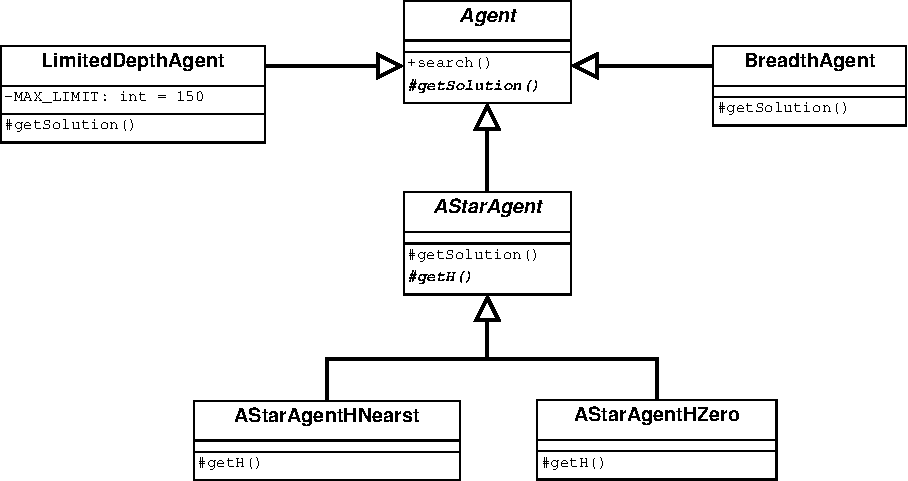
\includegraphics[scale=0.75]{uml.pdf}
    \caption{Digrama UML simplificado representando a hierarquia de classes entre os agentes 
    implementados.}
  \end{center}
\end{figure}

%%%%%%%%%%%%%%%%%%%%%%%%%%%%%%%%%%%%%%%%%%%%%%%%%%%%%%%%%%%%%%%%%%%%%%%%%%%%%%%%%%%%%%%%%%%%%%%%%%%%

\section{Heurística Utilizada}
\label{sec:h}

A heurística utilizada na implementação do método de busca do agente A* consiste na ideia natural de 
se calcular o número de passos que seriam necessários para o agente coletar a pepita mais próxima a 
ele, depois seguir dessa posição para a próxima pepita que esteja mais perto e assim sucessivamente 
até que se colete todas as pepitas desejadas, retornando finalmente à posição inicial da mina 
(confira a Figura~\ref{fig:mina}). Esse número total de passos entraria com sinal negativo e o total 
de ouro coletado (vezes $4n$) entraria com sinal positivo para dar o valor da função heurística: 
%
\begin{equation*}
h(n) = - \sum \text{(passos até pepitas mais próxima)} 
+ 4 n \sum \text{(pepitas)} \, .
\end{equation*}

O número de passos entre duas posições é calculado considerando que não existe nenhuma obstrução na 
mina entre elas, sendo portanto a soma das diferenças entre linhas e colunas. Se $x$ e $y$ são duas
posições na mina, então definimos a distância entre elas como:
%
\begin{equation*}
\|x - y\| = |\row(x)-\row(y)| + |\col(x) - \col(y)| \, .
\end{equation*}

Pelo fato de estarmos calculando distâncias diretas entre pontos na mina sem considerar as 
obstruções e estarmos usando uma estratégia gulosa (ir atrás da próxima pepita que esteja mais 
perto), a heurística definida deve ser adimissível\footnote{Confira a Seção~\ref{sec:conc} para uma
discussão sobre isso}.
%
\begin{figure}[htbp]
  \label{fig:mina}
  \begin{center}
    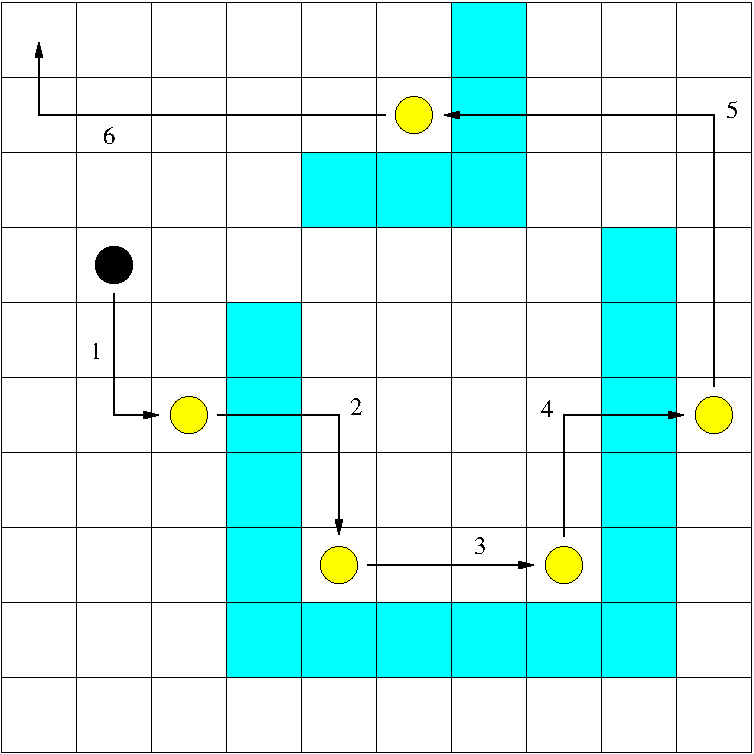
\includegraphics[scale=0.50]{mina.pdf}
    \caption{Representação da heurística utilizada. O agente (ponto preto) seguiria os caminhos 
    1, 2, 3, 4, 5 e 6 coletando todas as pepitas (pontos amarelos) e retornando a sua posição 
    inicial. Note que não há preocupação com as obstruções dos caminhos (quadrados em azul).}
  \end{center}
\end{figure}


%%%%%%%%%%%%%%%%%%%%%%%%%%%%%%%%%%%%%%%%%%%%%%%%%%%%%%%%%%%%%%%%%%%%%%%%%%%%%%%%%%%%%%%%%%%%%%%%%%%%

\section{Testes e Análise de Desempenho}
\label{sec:teste}

O programa foi testado usando 6 arquivos de entrada (os arquivos estão no diretório raiz 
numerados de um a seis) representando minas com dimensões diferentes. Medimos a pontuação obtida 
por cada um dos quatro agentes implementados, bem como o tempo de processamento. Os resultados são 
resumidos na Tabela~\ref{tab:res}.

\begin{table}
  \begin{center}
    \begin{tabular}{|c|c|c|c|c|}
      \hline 
      \bf $n$ & \bf P & \bf L & \bf U & \bf A \\
      \hline \hline 
      6 & 20 (0.006) & 34 (0.021) & 34 (0.020) & 34 (0.065) \\ \hline
      8 & 56 (0.029) & 70 (0.092) & 70 (0.067) & 70 (0.131) \\ \hline
      10 & 66 (0.095) & 118 (0.154) & 118 (0.109) & 118 (0.209) \\ \hline
      14 & 194 (2.288) & 306 (8.842) & 298 (0.355) & 304 (0.638) \\ \hline
      16 & 192 (16.497) & 412 (84.34) & 406 (3.895) & 412 (1.120) \\ \hline
      20 & 0 (15.963) & -- & -- & 726 (1.431) \\ \hline
      \end{tabular} 
      \caption{Pontuação obtida e tempo de processamento (entre parenteses em segundos) para cada
      um dos agentes implementados e para as seis entradas consideradas, representadas pela 
      dimensão da mina $n$. P = busca em profundidade, L = busca em largura, U = busca uniforme, 
      A = busca A*. Os traços indicam que nenhuma solução foi obtida com até 180 segundos de 
      processamento.}
      \label{tab:res}
  \end{center}
\end{table}

Os resultados da tabela claramente indicam que a busca em profundidade não obtém resultados ótimos
mesmo para instâncias pequenas. Apesar disso seu tempo de processamento é baixo. A busca em largura
obtém resultados ótimos mais é a que consome mais tempo para instâncias maiores. A busca uniforme 
e a busca A* são mais rápidas para instâncias maiores mas nem sempre obtém o ótimo. 
No caso $n = 16$, a busca A* atingiu o ótimo com o tempo de processamento bem inferior do que o da
busca em largura. No caso $n = 20$ apenas a busca A* conseguiu um resultado satisfatório.

%%%%%%%%%%%%%%%%%%%%%%%%%%%%%%%%%%%%%%%%%%%%%%%%%%%%%%%%%%%%%%%%%%%%%%%%%%%%%%%%%%%%%%%%%%%%%%%%%%%%

\section{Conclusões}
\label{sec:conc}

A implementação apresentada é baseada em bom projeto de classes, conforme apresentado na 
Seção~\ref{sec:classes}. Os resultados da Table~\ref{tab:res} indicam que os agentes se comportam
de maneira esperada, sendo A* o mais eficiente para instâncias maiores.

Alguns pontos devem ser considerados. Primeiro note que a busca do agente não é realizada com passos
de mesmo custo, pois em alguns casos ele perde um ponto ao se mover e, em outro, ganha $4n$ pontos
ao coletar uma pepita. Nesse caso~\cite{aima}, nem mesmo a busca em largura tem garantia de ser 
ótima. A busca uniforme, entretanto, deveria ser. Mas como a implementação evita estados repetidos, 
utilizando o algoritmo \verb|GRAPH-SEARCH| de~\cite{aima}, nesse caso, também não se tem a garantia 
de otimalidade. O mesmo acontece para a busca em profundidade, que é bem ineficiente dado que 
limitou-se a profundidade máxima para um valor baixo (\verb|MAX_LIMIT = 150|)a fim de se evitar 
tempos excessivos de processamento.

A busca A*, entretanto, deve ser ótima para \verb|GRAPH-SEARCH| desde que a heurística $h(n)$ seja
consistente. O fato de termos encontrado um resultado não ótimo para a instância $n = 14$ (304 
pontos contra 306 da busca em largura) indica que a heurística construída não é consistente e, 
portanto, também não deve ser adimissível.

%%%%%%%%%%%%%%%%%%%%%%%%%%%%%%%%%%%%%%%%%%%%%%%%%%%%%%%%%%%%%%%%%%%%%%%%%%%%%%%%%%%%%%%%%%%%%%%%%%%%

\begin{thebibliography}{99}
  \bibitem{aima} S.~Russell, P.~Norvig. {\it Artificial Intelligence -- A Modern Approach}. Segunda
  edição.
\end{thebibliography}

\end{document}

